\documentclass[10pt,svgnames]{beamer}
\graphicspath{{images/}}
\usepackage[utf8]{inputenc}
\usepackage[english,russian]{babel}
\usepackage{booktabs}
\usepackage{biblatex}
\usepackage{tabularx}


\usetheme[titleformat=smallcaps,
numbering=fraction,
subsectionpage=progressbar,
progressbar=frametitle]{metropolis}
\usecolortheme[light,accent=green]{solarized}
\setbeamercovered{transparent}
\newcommand{\dir}{\text{Dirichlet}}
\newcommand{\mult}{\text{Multinomial}}
\usetikzlibrary{arrows,decorations.pathmorphing,fit,positioning,automata}
\addbibresource{local.bib}



\title[CMTA 09] % (optional, use only with long paper }
{Word embeddings}

\subtitle
{Computational Methods for Text Analysis} % (optional)

\author%[Author, Another] % (optional, use only with lots of authors)
{Кирилл Александрович Маслинский}
% - Use the \inst{?} command only if the authors have different
%   affiliation.

\institute%[Universities of Somewhere and Elsewhere] % (optional, but mostly needed)
{НИУ ВШЭ Санкт-Петербург}
% - Use the \inst command only if there are several affiliations.
% - Keep it simple, no one is interested in your street address.

\date%[Short Occasion] % (optional)
{06.12.2021 / 09}

\subject{natural language processing, text mining}
% This is only inserted into the PDF information catalog. Can be left
% out. 



% If you have a file called "university-logo-filename.xxx", where xxx
% is a graphic format that can be processed by latex or pdflatex,
% resp., then you can add a logo as follows:

% \pgfdeclareimage[height=0.5cm]{university-logo}{university-logo-filename}
% \logo{\pgfuseimage{university-logo}}

% Delete this, if you do not want the table of contents to pop up at
% the beginning of each subsection:

\newcommand{\plate}[1]{\begingroup\setbeamercolor{background canvas}{bg=Beige}
  % \begin{frame}<beamer>{Outline}
  %   \tableofcontents[sectionstyle=show/hide,subsectionstyle=show/shaded/hide]
  % \end{frame}
  \begin{frame}[plain]
  \vfill
  \centering
  \begin{beamercolorbox}[sep=8pt,center,shadow=true,rounded=true]{title}
    \usebeamerfont{title}#1\par%
  \end{beamercolorbox}
  \vfill
  \end{frame}
  \endgroup
}

% \AtBeginSection[]
% {
%   \begin{frame}<beamer>[plain]{План}
%     \tableofcontents[sectionstyle=shaded,subsectionstyle=hide]
%   \end{frame}
% }

% \AtBeginSubsection[]
% {
%   \begin{frame}<beamer>[plain]{План}
%     \tableofcontents[sectionstyle=shaded,subsectionstyle=show]
%   \end{frame}
% }

\newcommand{\tb}[1]{\colorbox{yellow}{#1}\space}
\newcommand{\Sp}[1]{\colorbox{green}{#1}\space}
\newcommand{\Sn}[1]{\colorbox{red}{#1}\space}


\begin{document}

\begin{frame}
  \titlepage
\end{frame}

\section{Пространственное моделирование семантики}


\begin{frame}
  \frametitle{Word space}
  \begin{block}{Sch\"utze}
    Vector similarity is the only information present in Word Space:
    semantically related words are close, unrelated words are
    distant.
  \end{block}
  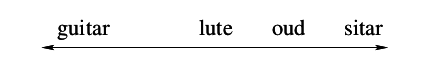
\includegraphics[width=.5\textwidth]{guitar1}
  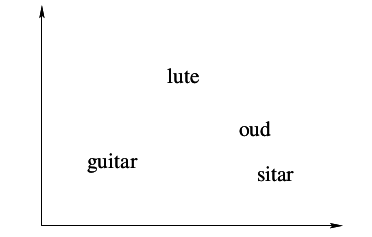
\includegraphics[width=.5\textwidth]{guitar2}
\end{frame}

\begin{frame}
  \frametitle{Пространственная метафора}
  Lakoff \& Johnson, Metaphors we live by, 1980

  Метафоры — основа всех абстрактных понятий. Язык вообще и языковое
  значение в частности построено на метафорах. 

  Первичные метафоры — непосредственно связаны с телесным опытом.
  \begin{itemize}
  \item Пространство:
    \begin{itemize}
    \item расположение
    \item направление
    \item близость (расстояние)
    \end{itemize}
  \end{itemize}
\end{frame}

\begin{frame}
  \frametitle{Геометрическая метафора языкового значения}
  В основе первичные метафоры:
  \begin{itemize}
  \item похожее = близкое
  \item сущность = место (понятие = место)
  \end{itemize}
  \begin{block}{Геометрическая метафора языкового значения:}
    Значения — это точки в семантическом пространстве, семантическое
    сходство — расстоние между точками в этом пространстве.
  \end{block}
\end{frame}

\begin{frame}
  \frametitle{Дистрибутивная семантика}
  \begin{block}{Дистрибутивная гипотеза}
    Слова со сходными дистрибутивными свойствами обладают сходным значением.
  \end{block}
  Способы представить дистрибутивное сходство:
  \begin{itemize}
  \item соседствуют с одними и теми же словами
  \item употребляются в одних и тех же документах
  \item ...
  \end{itemize}
\end{frame}


\begin{frame}
  \frametitle{Пространственные модели значения}
  \begin{itemize}
  \item LSA/LSI (Latent Semantic Analysis/Indexing) [1988]
  \item word2vec [2013]
  \item ELMo/BERT/GPT-2/GPT-3 [2017—2020]
  % \item HAL (Hyperspace analog to language)
  % \item RP/RI (Random projection/indexing)
  \end{itemize}
  Все они по-разному реализуют одну и ту же идею:
  \begin{itemize}
  \item геометрическая метафора значения
  \item дистрибуитвный метод: построение пространства на основе
    информации о контекстах слов
  \item моделируют семантическую близость: смысл в модели имеет только расстояние, но не измерения пространства
  \end{itemize}
\end{frame}

\begin{frame}
  \frametitle{Выводы о дистрибутивной семантике}
  В «семантическом пространстве» (word space):
  \begin{itemize}
  \item \textbf{Имеет смысл} анализ расстояния между \alert{близкими} по значению словами.
  \item \textbf{Не имеет смысла} анализ расстояния между не связанными по
    значению словами (удаленными областями в word space).
    \textit{Что общего между вороном и конторкой}?
  \end{itemize}
\end{frame}

\section{Word embeddings}

\begin{frame}
  \frametitle{Терминология}
  \begin{description}
  \item[Word embeddings] — dense representations of words in a
    low-dimensional vector space
  \item[neural word embeddings] word embeddings learned by a neural
    network
  \end{description}
  Alternate terms: distributional semantic model/semantic vector space/word space
\end{frame}

\plate{Serendipity:\\ $king-man+woman \approx queen$
  \bigskip
\includegraphics<1>[width=.8\textwidth]{kmw}
\includegraphics<2>[width=.6\textheight]{analogy-3d}
}

\begin{frame}
  \frametitle{Семантическая алгебра}
  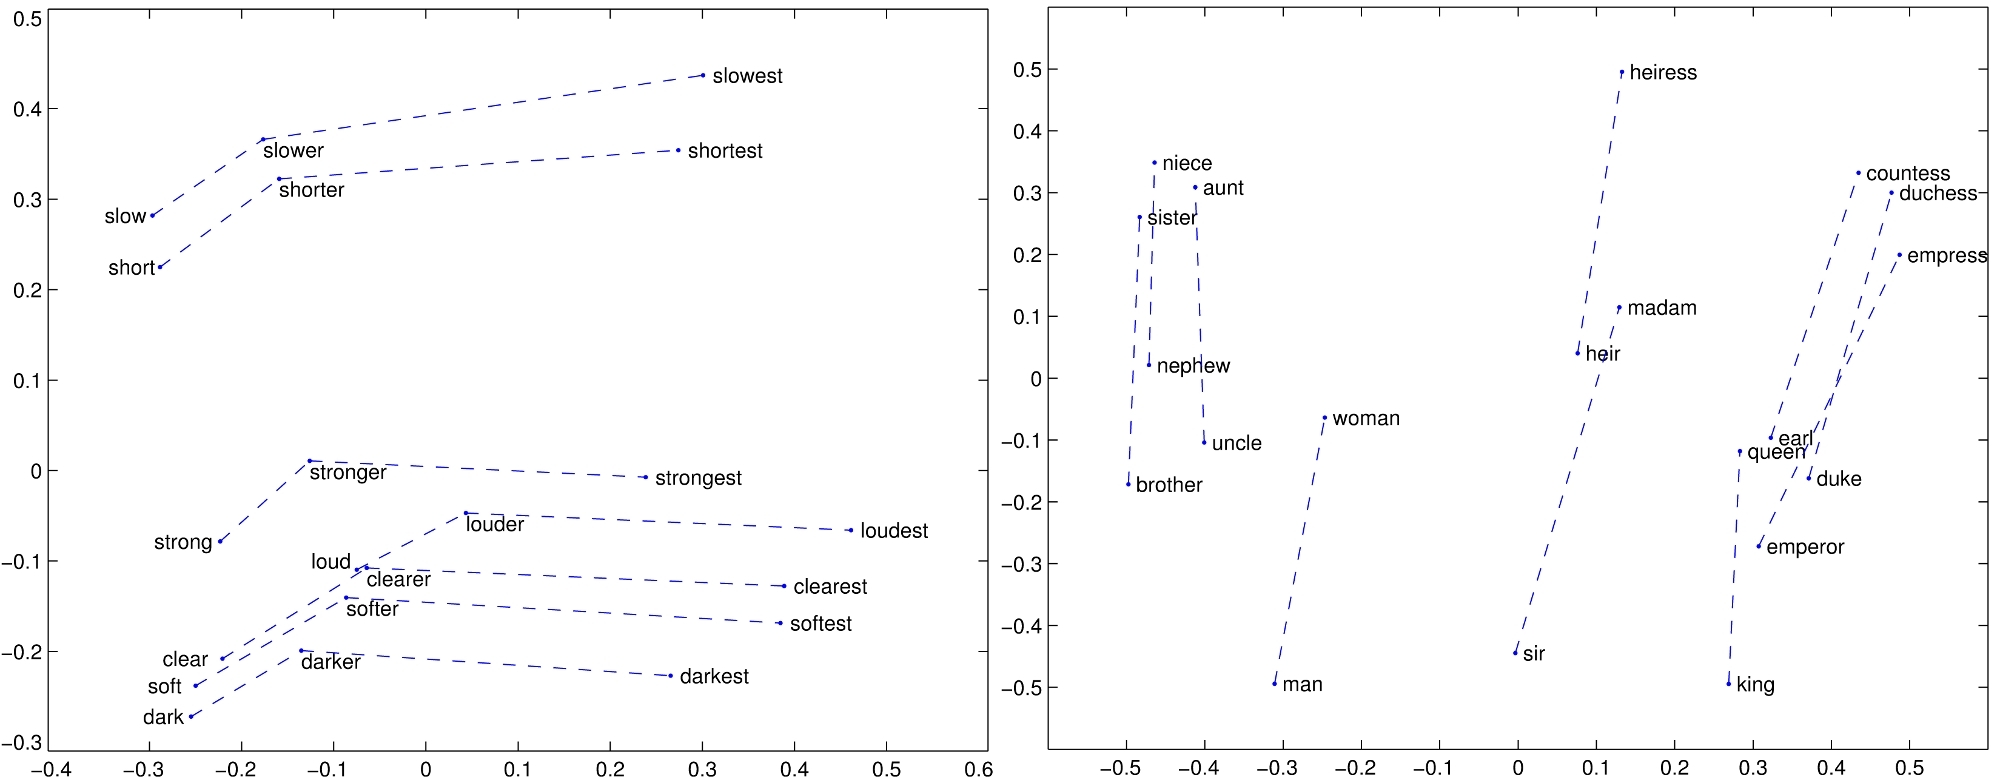
\includegraphics[width=\textwidth]{comparatives}
\end{frame}

\begin{frame}
  \frametitle{Прорыв и фавориты}
  \begin{description}
  \item[word2vec] Mikolov et al. in 2013 
  \item[GloVe] Pennington et al. 2014
  \end{description}
\end{frame}

\begin{frame}
  \frametitle{Нейронные сети и Deep Learning Revival}
  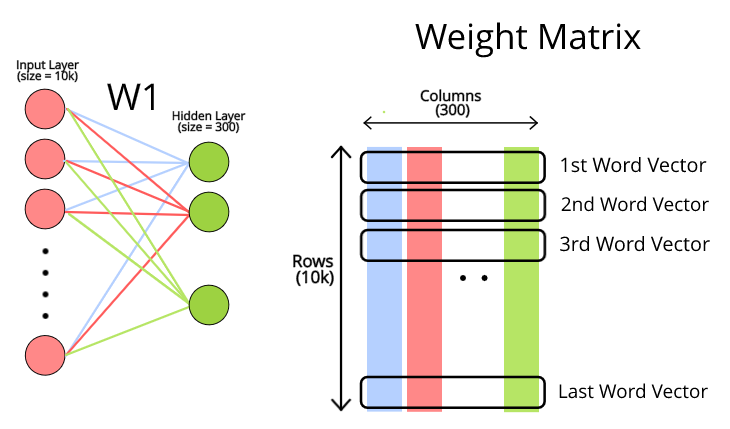
\includegraphics[width=\textwidth]{w2v-arch}
\end{frame}

% Their main benefit arguably is that they don't require expensive
% annotation, but can be derived from large unannotated corpora that
% are readily available. Pre-trained embeddings can then be used in
% downstream tasks that use small amounts of labeled data.

% word2vec and GloVe are geared towards producing word embeddings that
% encode general semantic relationships, which are beneficial to many
% downstream tasks

\begin{frame}
  \frametitle{Успех и польза}
  Unsupervised method:
  \begin{itemize}
  \item[->] большой неаннотированный корпус текстов
  \item[->] pre-trained embeddings
  \item[->] применение к небольшим массивам размеченных данных
  \end{itemize}
\end{frame}

\begin{frame}
  \frametitle{Применения word2vec}
  \includegraphics<1>[width=\textwidth]{semantic_change}
  \includegraphics<2>[width=\textwidth]{hamilton-drift}
  % добавить картинки из Гамильтона

  \only<1>{Hamilton W. L., Leskovec J., Jurafsky D. Diachronic Word Embeddings Reveal Statistical Laws of Semantic Change //Proceedings of the 54th Annual Meeting of the Association for Computational Linguistics (Volume 1: Long Papers). – 2016. – С. 1489-1501.
}
  \only<2>{Hamilton W. L. et al. Inducing domain-specific sentiment lexicons from unlabeled corpora //Proceedings of the Conference on Empirical Methods in Natural Language Processing. Conference on Empirical Methods in Natural Language Processing. – NIH Public Access, 2016. – Т. 2016. – С. 595.}
\end{frame}

\plate{SGNS — Skip-gram with negative sampling aka word2vec

  \bigskip
  \hrule
  \bigskip
  
  Illustrations from: http://jalammar.github.io/illustrated-word2vec/

  Русский перевод: https://habr.com/ru/post/446530/
}


\begin{frame}
  \frametitle{Embeddings: vectors for words}
  \centering
  \includegraphics<1>[width=\textwidth]{king-colored-embedding}
  \includegraphics<2>[width=\textwidth]{king-man-woman-embedding}
  \includegraphics<3>[width=\textwidth]{queen-woman-girl-embeddings}
  \includegraphics<4>[width=\textwidth]{king-analogy-viz}
\end{frame}


\begin{frame}
  \frametitle{Языковая модель: задача предсказания слова}
  \includegraphics<1>[width=\textwidth]{thou-shalt-_}
  \includegraphics<2>[width=\textwidth]{language_model_blackbox}
  \includegraphics<3>[width=\textwidth]{neural-language-model-prediction}
\end{frame}

\begin{frame}
  \frametitle{Метод скользящего окна}
  \includegraphics<1>[width=\textwidth]{lm-sliding-window-2}
  \includegraphics<2>[width=\textwidth]{lm-sliding-window-3}  
\end{frame}

\begin{frame}
  \frametitle{Skipgram}
  \includegraphics<1>[width=\textwidth]{continuous-bag-of-words-example}
  \includegraphics<2>[width=\textwidth]{skipgram-sliding-window-samples}    
  \includegraphics<3>[width=\textwidth]{skipgram-sliding-window-5}    
\end{frame}

\begin{frame}
  \frametitle{Обучение модели}
  \includegraphics<1>[width=\textwidth]{skipgram-language-model-training-5}  
\end{frame}

\begin{frame}
  \frametitle{Negative sampling}
  \includegraphics<1>[width=\textwidth]{language-model-expensive}
  \includegraphics<2>[width=\textwidth]{predict-neighboring-word}    
  \includegraphics<3>[width=\textwidth]{are-the-words-neighbors}      
\end{frame}

\begin{frame}
  \frametitle{Noise-contrastive estimation}
  \includegraphics<1>[width=\textwidth]{word2vec-training-dataset}
  \includegraphics<2>[width=\textwidth]{word2vec-smartass-model}    
  \includegraphics<3>[width=\textwidth]{word2vec-negative-sampling}        
  \includegraphics<4>[width=\textwidth]{word2vec-negative-sampling-2}        
\end{frame}

\begin{frame}
  \frametitle{SGNS: SkipGram with Negative Sampling}
  \includegraphics<1>[width=\textwidth]{skipgram-with-negative-sampling}  
\end{frame}

\section{Обучение модели word2vec (SGNS)}

\begin{frame}
  \frametitle{Обучение word2vec}
  \includegraphics<1>[width=\textwidth]{word2vec-embedding-context-matrix}
  \includegraphics<2>[width=\textwidth]{word2vec-lookup-embeddings}    
  \includegraphics<3>[width=\textwidth]{word2vec-training-dot-product}        
  \includegraphics<4>[width=\textwidth]{word2vec-training-dot-product-sigmoid}          
  \includegraphics<5>[width=\textwidth]{word2vec-training-error}          
  \includegraphics<6>[width=\textwidth]{word2vec-training-update}          
\end{frame}

\section{Параметры модели word2vec}

\begin{frame}
  \frametitle{Размер контекстного окна}
  \includegraphics<1>[width=\textwidth]{word2vec-window-size}  
\end{frame}

\begin{frame}
  \frametitle{Количество отрицательных примеров}
  \includegraphics<1>[width=\textwidth]{word2vec-negative-samples}    
\end{frame}

\section{Word embeddings and distributional semantic models}

\begin{frame}
  \frametitle{Сравнение с дистрибутивными моделями}
  \begin{tabularx}{1.0\linewidth}{|X|X|X|X|}
    \hline
    \textbf{модели} & \textbf{контекст} & \textbf{тип отношения} &
                                                                   \textbf{пример} \\
    \hline
     LSA, pLSA, LDA & документ & semantic relatedness & boat — water
    \\
    \hline
     word embeddings, HAL, Random indexing, BEAGLE & слова & semantic
                                                             similarity
                                                                 &
                                                                   boat
                                                                   —
                                                                   ship
    \\
    \hline
  \end{tabularx}
\end{frame}


\begin{frame}
  \frametitle{Как мы и думали, никакой разницы!}
  \fullcite{levy2014neural}
\end{frame}




\section{word2vec: секрет успеха}



\begin{frame}
  \frametitle{Pre-processing}
  \begin{itemize}
  \item Dynamic context window:  $decay = 1/distance$
  \item Subsampling frequent words: randomly delete words that are too
    common
  \item Deleting rare words
  \end{itemize}
\end{frame}

\begin{frame}
  \frametitle{Association metric}
  \begin{itemize}
  \item Shifted PMI $SPPMI(w, c) = max(pmi(w,c) - log(k), 0)$
  \item Context distribution smoothing
    $$
    pmi(w,c) = log \frac{p(w,c)}{p(w)p_{\alpha}(c)}, where
    p_{\alpha}(c) = \frac{f(c)^{\alpha}}{\sum_{c} f(c)^{\alpha}}, \alpha = \frac{3}{4}
    $$
  \end{itemize}
\end{frame}


\begin{frame}
  \frametitle{Levy et al 2015 takeaways}
  \begin{itemize}
  \item 
    Hyperparameters vs. algorithms:
    
    Hyperparameter settings are often more important than algorithm choice.
    No single algorithm consistently outperforms the other methods.
  \item Hyperparameters vs. more data:
    
    Training on a larger corpus helps for some tasks.
    In 3 out of 6 cases, tuning hyperparameters is more beneficial.
  \end{itemize}
\end{frame}

\begin{frame}
  \frametitle{Debunking prior claims}
  
  \begin{enumerate}
  \item Are embeddings superior to distributional methods?

    With the right hyperparameters, no approach has a consistent
    advantage over another.
  \item Is GloVe superior to SGNS?

    SGNS outperforms GloVe on all tasks.
  \item Is CBOW a good word2vec configuration?

    CBOW does not outperform SGNS on any task.
  \end{enumerate}
\end{frame}

\section{Explaining word embeddings}

\begin{frame}
  \frametitle{Pointwise mutual information}
  PMI

  $$
  pmi(x;y) = log \frac{p(x,y)}{p(x)p(y)} = log \frac{p(x|y)}{p(x)} =
  log \frac{p(y|x)}{p(y)}
  $$

  Positive PMI

    $$
    ppmi(x;y) = max(pmi(x;y),0)
    $$    
\end{frame}

\begin{frame}
  \frametitle{Четыре вида сходства}
  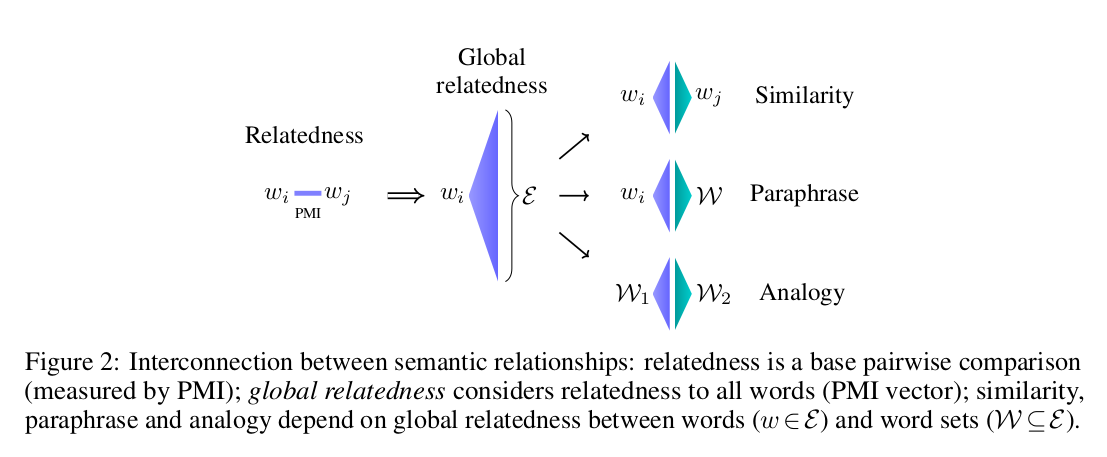
\includegraphics[width=\textwidth]{sem-rels}\footnote{Allen, C.,
    Balazevic, I., \& Hospedales, T. (2019). What the vec? towards
    probabilistically grounded embeddings. Advances in Neural
    Information Processing Systems, 32, 7467-7477.}
\end{frame}

\end{document}
